
\chapter{Project Overview}
\label{sect:goals}
{%\hypersetup{linkcolor=black}
\startcontents[chapters]
\printcontents[chapters]{}{1}{}
}
\noindent\\
This chapter discusses the the project's requirements, goals, and structure.

\section{Project Deliverables}
The project's deliverables are split into two sections: core deliverables (CD) -- each deliverable must be satisfied for the project to be a minimum viable product (MVP), and extended deliverables (ED) -- deliverables that are not required for a MVP -- features that only improve upon an existing feature.

\subsection{Core Deliverables (CD)}
The project's core deliverables are described below.
\begin{enumerate}[leftmargin=2\parindent, label=\bfseries CD\arabic*]
\item{\textbf{Design a compact 16-bit RISC instruction set architecture.}\\
The instruction set will be the primary interface to control the processor from software. An instruction set will be required to implement the custom multi-core communication interface.

It was decided to design a new instruction set rather than to extend an existing architecture as this will increase my knowledge of the constraints to consider when designing instruction sets and processors.
}
\label{cd:isa}

\item{\textbf{Design and implement a Verilog RISC core that implements the ISA in \ref{cd:isa}.}\\
The Verilog RISC core will be able to run software program written for the instruction set architecture.
}\label{cd:core}

\item{\textbf{Design and implement an on-chip interconnect for multi-core processing (2 to 32 cores) using the RISC core from \ref{cd:core}.}\\
The interconnect will be a chief requirement to enable multi-core communication. The interconnect should support up to 32 cores, however FPGA implementation constraints may limit this due to limited resources.

The interconnect will control communication between the cores to enable software parallelism.
}\label{cd:interconnect}

\item{\textbf{Analyse performance of serial and parallel software algorithms, such as parallel DFT, on the processor.}\\
To evaluate the effectiveness of the developed solution, a serial and parallel implementation of a simple computing algorithm (parallel reduction, sorting) will be ran on the processor and it's performance analysed. Effectiveness will be rated on total algorithm run-time and the speed-up gained by adding more cores.
}\label{cd:software}

\item{\textbf{Allow the RISC core to be easily compiled to multiple FPGA vendors (Xilinx, Altera).}\\
The developed solution should be generic and portable to allow it to be used across a wide-range of FPGA vendors and devices.

Verilog is a generic implementation-independent hardware-description language and so designing implementation specific modules is recommended.

A key consideration for this requirement is to consider the varying hard IP provided by the FPGA vendors (such as BRAM, ethernet, and PCIe \cite{xilinxbram,alterabram}). To overcome this problem, the developed Verilog code will conditionally compile where vendor specific requirements are present.
}\label{cd:vendor}
\end{enumerate}

\subsection{Extended Deliverables (ED)}
The project's extended deliverables are described below.
\begin{enumerate}[leftmargin=2\parindent, label=\bfseries ED\arabic*]
    \item{Design a RISC core with an instructions-per-clock (IPC) rating of at least 1.0 (a single-cycle CPU).}
\label{ed:ipc}
    \item{Design a RISC core with a pipe-lined data path to increase the design's clock speed.}\label{ed:pipeline}
    \item{Design a scalable multi-core interconnect supporting arbitrary (more than 32) RISC core instances (manycore) using Network-on-Chip (NoC) architecture.}\label{ed:scale}
    \item{Design a compiler-backend for the PRCO304 \cite{prco304} compiler to support the ISA from \ref{cd:isa}. This will make it easier to build complex multi-core software for the processor.}\label{ed:compiler}
    \item{The RISC core can communicate to peripherals via a memory-mapped addresses using the Wishbone bus.}\label{ed:mmu}
    \item{Implement various memory-mapped peripherals such as UART, GPIO, LCD, to aid visual representation of the processor during the demonstration viva.}\label{ed:peripherals} 
    \item{Store instruction memory in SPI flash.}\label{ed:flash}
    \item{Reprogram instruction memory at runtime from host computer.}\label{ed:program}
    \item{Processor external debugger using host-processor link.}\label{ed:debug}
\end{enumerate}

\section{Project Timeline}
\label{sect:timeline}
\subsection{Project Stages}
The project is split up into many stages to aid planning and management of the project. There are 8 unique stage areas: 1. Inital project conception; 2 Basic RISC core development; 3. Extended RISC core development; 4. Multi-core development; 5. Processor quality-of-life (QoL) improvements; 6. Compiler development; 7. Demo preparation, and 8. Final report.

The project stages are shown in Table \ref{tb:stages}.

\begin{table}[h]
    \small
    \begin{tabularx}{\textwidth}{|l|l|l|l|X|}
    \hline
    Stage & Title & Start Date & Core & Status
    \\ \specialrule{2pt}{-2pt}{0pt}
    1.0 & Research & Feb 04 & x & Completed
    \\ \hline
    1.1 & Requirement gathering/review & Feb 11 & x & Completed
	\\ \hline
    1.1 & Processor specification, architecture, ISA & Feb 18 & x & Completed
	\\ \hline
    1.2 & Stage/Time Allocation Planning & Feb 25 & x & Completed
    \\ \specialrule{2pt}{-2pt}{0pt}
    2.1 & Decoder, Register Set, impl \& integration & Feb 25 & x & Completed
	\\ \hline
    2.2 & Register set impl \& integration & Mar 04 & x & Completed
	\\ \hline
    2.3 & Local memory impl \& integration & Mar 11 & x & Completed
    \\ \specialrule{2pt}{-2pt}{0pt}
    3.1 & Memory mapped register layout \& impl & Apr 01 &  & On-going
	\\ \hline
    3.2 & Wishbone peripheral bus connected to MMU & Apr 08 &  & On-going
	\\ \hline
    3.3 & Pipeline implementation and verification & Apr 15 &  & On-going
	\\ \hline
    3.4 & Cache memory design \& impl & \st{Apr 22} &  & Cancelled
    \\ \specialrule{2pt}{-2pt}{0pt}
    4.1 & Multi-core communication interface & Jun 05 & x & Planned
	\\ \hline
    4.2 & Shared-memory controller & Jun 05 & x &Planned
	\\ \hline
    4.3 & Scalable multi-core interface (10s of cores) & Jul 01 & x & Planned
	\\ \hline
    4.4 & Multi-core example program (reduction) & Jul 10 & x & Planned
    \\ \specialrule{2pt}{-2pt}{0pt}
    5.1 & SPI-FPGA interface for OTG programming & \st{TBD} &  & Cancelled
	\\ \hline
    5.2 & FPGA-PC interfacing & \st{TBD} &  & Cancelled
	\\ \hline
    5.3 & FPGA-PC debugging (instruction breakpoints) & \st{TBD} & & Cancelled
    \\ \specialrule{2pt}{-2pt}{0pt}
    6.1 & Compiler backend for vmicro16 & TBD &  & Unknown
	\\ \hline
    6.2 & Compiler support for multi-core codegen & TBD &  & Unknown 
    \\ \specialrule{2pt}{-2pt}{0pt}
    7.1 & Wishbone peripherals for demo & Aug 01 & x & Planned
    \\ \specialrule{2pt}{-2pt}{0pt}
    8.1 & Final Report & Jun 05 & x & Planned
	\\ \hline    \end{tabularx}
    \caption{Project stages throughout the life cycle of the project.}
    \label{tb:stages}
\end{table}

\subsection{Project Stage Detail}
\subsubsection{Stages 1.0 through 1.2 --  Research and Project Conception}
These stages cover initial research of existing problems and solutions in the multiprocessor area. 
The instruction set architecture is also proposed that later stages will implement.

\subsubsection{Stages 2.1 through 2.3 -- Processor module Design, Implementation, and Integration}
These stages cover the design, implementation, and integration of key processor core modules such as the instruction decoder, register sets and local memory.
Integration of all the modules is a challenging task because some modules have both asynchronous and synchronous signals that need to be timed correctly in order for other modules to receive valid data. An example of this is the register set which has asynchronous read ports that are later clocked in the instruction decode stage.

\subsubsection{Stages 3.1 through 3.4 -- Advanced Processor Implementation}
These stages add advanced features to the processor to provide a more functional product. Although these stages are classified as extended, their technical requirement to design and implement is not great and so are have time allocations in the project schedule. The extended features that these stages introduce are: pipelined processor stages -- to drastically increase processor performance; provide a memory-mapped peripheral interface through the MMU; provide a Wishbone master interface to the MMU -- allowing external peripherals such as GPIO and LCD displays to be utilised in a modular fashion; and to implement a cache memory for each processor core.

\subsubsection{Stages 4.1 through 4.4 -- Multiprocessor Functionality}
These stages are dedicated to adding multiprocessor functionality using a loosely coupled architecture to the processor.

\subsubsection{Stages 5.1 through 5.3 -- Debugging Features}
These stages cover debugging features and are classified as extended due to the large development time required to implement them as well as not being related to multiprocessor systems.

\subsubsection{Stages 6.1 through 6.2 -- Compiler Backends}
These stages cover the implementation of a compiler backend to ease software writing and programming of the processor.

\subsubsection{Stage 7.1 -- Wishbone Peripherals}
Additional Wishbone peripherals, such as SPI and timers will be added to produce a more useful multiprocessor system.

\subsubsection{Stage 8.1 -- Final Report}
This stage is dedicated to the final report write-up. It is expected to be an iterative task that is active throughout the lifespan of the project.

\subsection{Timeline}
The project stages from Table \ref{tb:stages} are displayed below in a Gantt chart.

\begin{figure}[h]
\centering
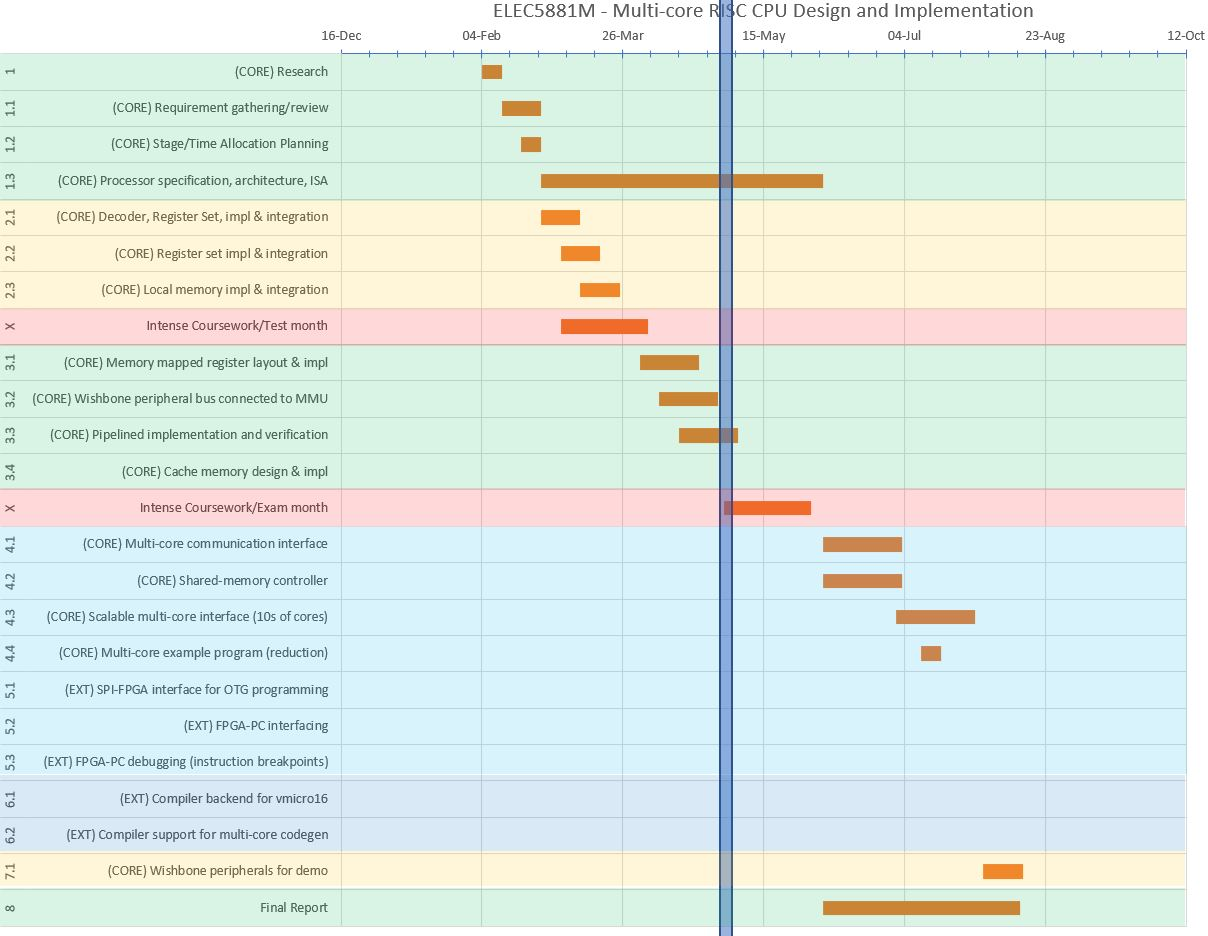
\includegraphics[width=13cm]{../img/week2_gantt}
\caption{Project stages in a Gantt chart.}
\label{fig:gantt}
\end{figure}


\section{Resources}
This section describes the hardware and software resources required to fulfil the project. 

\subsection{Hardware Resources}
Core deliverable \ref{cd:vendor} requires the designed RISC core to be implemented and demonstrated on multiple FPGA devices.  Although my design should synthesise for physical IC implementation, due to high costs and lengthy production times, it is not a primary development target. 
Due to having past experience with Xilinx FPGAs from my placement work and experience with Altera from university modules it was decided to target the Xilinx Spartan 6 XC6SLX9 and the Altera Cyclone V.

\subsubsection{Terasic DE1-SoC Development Board}
The Terasic DE1-SoC development board features a large Cyclone V FPGA and many peripherals, such as seven-segment displays, 64 MB SDRAM, ADCs, and buttons and switches, which will aid demonstration of the project. The development board is available through the university so the cost is negligible. \cref{fig:de1soc} shows the peripherals (green) available to the FPGA.

\begin{figure}[h]
\centering 
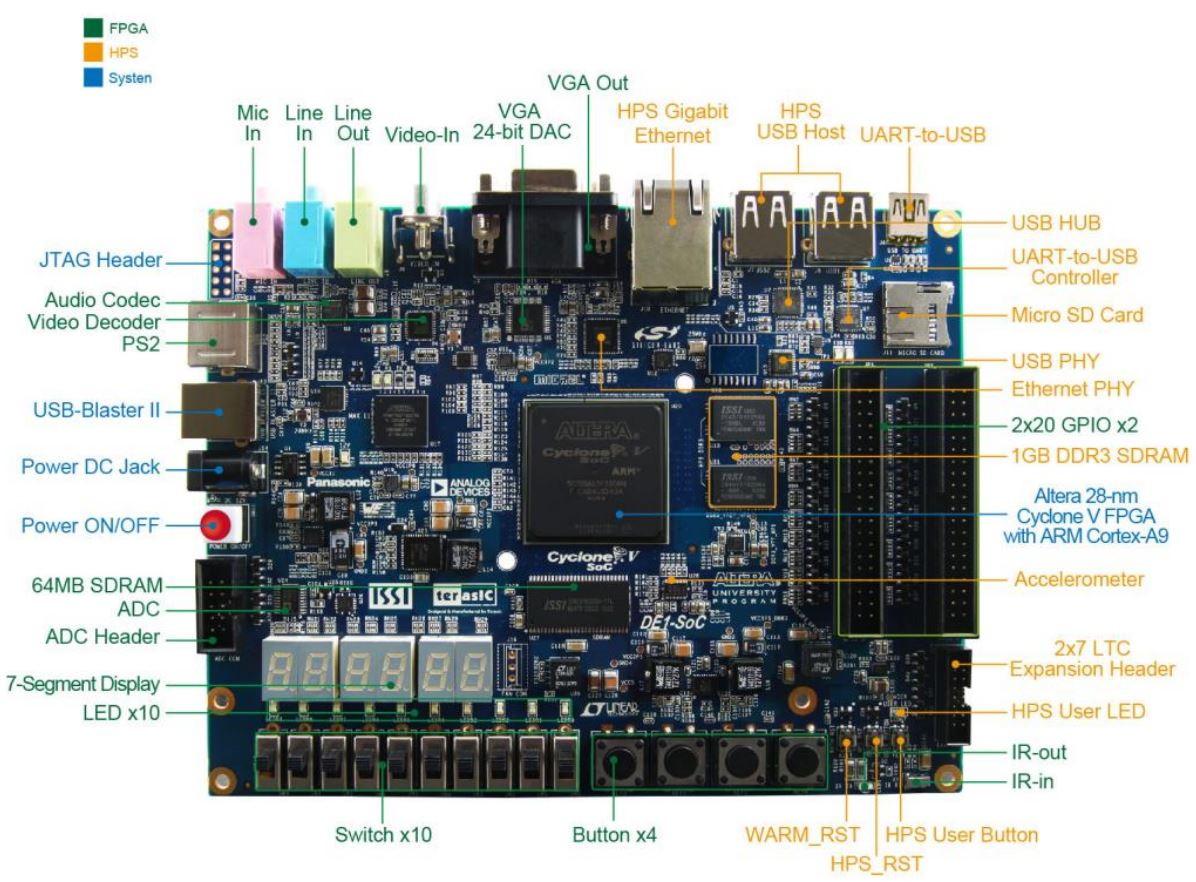
\includegraphics[width=10cm]{../img/de1soc}
\caption{Terasic DE1-SoC development board featuring the Altera Cyclone V FPGA and many peripherals. Image source: \cite{de1soc}.}
\label{fig:de1soc}
\end{figure}

\subsubsection{Minispartan 6+ FPGA Development Board}
The Minispartan 6+ is a hobbyist FGPA development board with fewer peripherals than the DE1-SoC. The board features a Xilinx Spartan 6 XC6LX9 which has far fewer resources than the DE1-SoC's Cyclone V however it's simplicity and my familiarity with  Xilinx's software suite will speed up development. The development board is shown in \cref{fig:minispartan}.

\begin{figure}[h]
\centering 
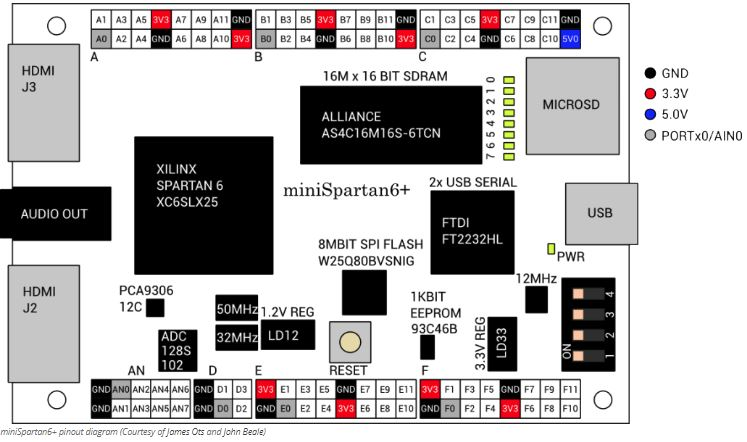
\includegraphics[width=10cm]{../img/minispartan}
\caption{Minispartan-6+ development board featuring the Xilinx Spartan 6 XC6SLX9. Note that the XC6SLX9 and XC6SLX25 FPGAs share the same board. Image source: \cite{scarabhardware}.}
\label{fig:minispartan}
\end{figure}

\subsection{Software Resources}
\subsubsection{Intel Quartus}
Intel Quartus Prime is a paid-for SoC, CPLD, and FPGA software suite targeting Intel's Stratix, Arria, and Cyclone based FPGAs. The university provides student licences which will be used via VPN.


\subsubsection{Xilinx ISE Webpack}
Xilinx ISE Webkpack is Xilinx's free software suite for FPGA development for Spartan 6 based FPGAs.
Due to ISE's intuitive and fast work flow, most of the initial simulation and verification processes will be performed using ISE. This will greatly improve development times.

\subsubsection{Verilator}
Verilator is an open-source Verilog to C++ transpiler which provides a C++ interface to simulate Verilog modules and read/write values similar to a test bench. Verilator will be used for specific modules within the RISC core such as the ALU and decoder as Verilator is useful when performing exhaustive verification.

\section{Legal and Ethical Considerations}
The RISC core is designed to be used as an academic research and educational tool to aid learning and understanding of RISC and multi-core machines. It should not be use for roles where mission critical or safety is a factor. 

The processor does not provide any memory protection features and any software running on the processor has full access to all memory.

The processor does not store/track/predict software instructions. The processor uses pipelining techniques to improve performance which results in future instructions entering the pipeline even if the software's logical sequence does not include these instructions. This could result in security vulnerabilities similar to Intel's Spectre vulnerability \cite{kocher2018spectre}.
